\documentclass[a4paper, 12pt]{article}

\usepackage[portuges]{babel}
\usepackage[utf8]{inputenc}
\usepackage{amsmath}
\usepackage{indentfirst}
\usepackage{blindtext}
\usepackage{graphicx}
\usepackage[hidelinks]{hyperref}
\usepackage{gensymb}
\usepackage[usenames, dvipsnames]{xcolor}

\author{Igor Abreu da Silva}

\title{Trabalho Final de Sistemas Lineares I}

\begin{document}
	
	\begin{titlepage}
		\begin{center}
			\huge{Universidade Federal do Rio de Janeiro}
			\vspace{95pt}

			\large{Trabalho Final de Sistemas Lineares I}
			\vspace{160pt}
		\end{center}
		
		\begin{flushleft}
			\begin{tabbing}
				Alunos\qquad\qquad\= Igor Abreu da Silva\\
				DRE\> 112053874 \\
				Curso\> Engenharia Eletrônica \\
				Turma\> 2016/2 \\
				Professor\> Natanael Nunes de Moura Junior \\
			
			\end{tabbing}
			
		\end{flushleft}
		
		\begin{center}
			\vspace{\fill}
			Rio de Janeiro, 09 de Dezembro de 2016
		\end{center}
	\end{titlepage}


	\newpage
	\tableofcontents
	\listoffigures
	\thispagestyle{empty}
	
	\newpage
	\pagenumbering{arabic}
	\section{Conhecimentos}
		\subsection{Leis de kirchhoff}\label{kirchhoff}
		\subsubsection{Lei das Correntes}
			A soma das correntes em um nó e igual a zero.
		\subsubsection{Lei das Tensões}
			A soma das tensões em uma malha fechada é nula.
		\subsection{Propriedades de Laplace}
			\subsubsection{Propriedade da diferenciação}\label{derivada}
			\[
			x(t) \Rightarrow X(S) \rightarrow \int_{0}^{+\infty} \frac{dx}{dt}e^{-st}dt \Rightarrow s\int_{0}^{\infty} x(t)e^{-st}dt - x(0^{-}) = sX(s) - x(0^{-})
			\]
		\subsection{Função de Transferência}
		É a relação da saida sobre a entradas $H(S) = \frac{Y(S)}{X(S)}$			
		\subsection{Pólos e Zeros}\label{zero}
		Pólos são valores de \textbf{s} onde temos uma indefinição na função de transferência, ou seja quando o denominador é zero.

		
		Zeros são todos os valores de \textbf{s} que zera a função de transferência, em outras palavras fazem com que o numerador seja igual a zero.
		\subsection{Diagrama de Bode}\label{bode}
		\[
		H(S) = \frac{Y(s)}{X(S)} \Rightarrow \frac{\textcolor{blue}{k}(\textcolor{red}{s+a_{1}})}{\textcolor{Brown}{s}(\textcolor{Violet}{s+b_{1}})(\textcolor{Orange}{s^{2}+b_{2}s+b_{3}})}
		\]
		Organizando esta equação, temos:
		\[
		 \frac{\textcolor{blue}{k}(\textcolor{red}{a_{1}(\frac{s}{a_{1}}+1)})}{\textcolor{Brown}{s}\textcolor{Violet}{b_{1}}\textcolor{Orange}{b_{3}}(\textcolor{Violet}{\frac{s}{b_{1}}+1})(\textcolor{Orange}{\frac{s^{2}}{b_{3}}+\frac{b_{2}s}{b_{3}}+1})}
		\]		
		Com isso, teremos:
		\[
		|H(jw)| = 		 \frac{\textcolor{blue}{k}(\textcolor{red}{a_{1}(\frac{jw}{a_{1}}+1)})}{\textcolor{Brown}{jw}\textcolor{Violet}{b_{1}}\textcolor{Orange}{b_{3}}(\textcolor{Violet}{\frac{jw}{b_{1}}+1})(\textcolor{Orange}{\frac{(jw)^{2}}{b_{3}}+\frac{b_{2}jw}{b_{3}}+1})}
		\]
		Por questões praticas, com o objetivo de facilitar as contas, adaptaremos essa função para utilizar como a representação magnitude de decibel, logo teremos:\\
		
		\[20log(|H(jw)|) = 20log(|\frac{ka_{1}}{b_{1}b{3}}|) + 20log(|\frac{jw}{a_{1}}+1|) - 20log(|jw|) -20log(|\frac{jw}{b_{1}}+1|) 
		\]
		\[
		- 20log(|\frac{(jw)^{2} + b_{2}jw}{b_{3}}+1|)
		\]
		Como fase, teremos: 
		
		\[
		\angle H(jw) = \angle (\frac{jw}{a_{1}}+1) - \angle jw - \angle (\frac{jw}{b_{1}}+1) - \angle (\frac{(jw)^{2} + b_{2}jw}{b_{3}}+1)
		\]
		
		\textbf{Para o termo constante: $\frac{ka_{1}}{b_{1}b{3}}$}
		
		Modulo começa em $20log(\frac{ka_{1}}{b_{1}b{3}})$ 
		
		Fase será $\pi, \frac{ka_{1}}{b_{1}b{3}} > 0$ ou $0, \frac{ka_{1}}{b_{1}b{3}} \leq 0$\\ 
		
		\textbf{Termo: $j\omega$} 
		
		Modulo -20db/dec (Pólo) ou +20db/dec (zero)
		
		Fase $-arctg(\frac{w}{0})$, ou seja, $-90^{o}$ (pólo) $+90^{o}$ (zero)\\
		
		\textbf{Primeira Ordem: $\frac{jw}{b_{1}}+1$} 
		
		Modulo, começando na frequência de corte $b_{1}$, -20db/dec (Pólo) ou +20db/dec (zero)
		
		Fase $0_{o}$ em $\frac{b_{1}}{10}$, $-45^{o}$ (pólo) $+45^{o}$ (zero) em $b_{1}$ e por fim $-90^{o}$ (pólo) $+90^{o}$ (zero) em $100b_{1}$\\
		
		\textbf{Segunda Ordem: $\frac{(jw)^{2} + b_{2}jw}{b_{3}}+1$} 
		
		Modulo, começando na frequência de corte $b_{3}$, -40db/dec (Pólo) ou +40db/dec (zero)
		
		Fase $0_{o}$ em $\frac{b_{3}}{10}$, $-90^{o}$ (pólo) $+90^{o}$ (zero) em $b_{3}$ e por fim $-180^{o}$ (pólo) $+180^{o}$ (zero) em $100b_{3}$\\		
	\newpage
	\section{Quest\~{a}o 1}
		Nesta sessão serão resolvidas todas as partes necessárias para encontrar as funções/utilidades de cada um dos circuitos, bem como a analise de resposta a determinados sinais e todos os itens solicitados na \textbf{Questão 1} do trabalho final de sistemas lineares.
		
		O primeiro passo é modelar cada circuito, essa modelagem utilizara as leis de kirchhoff explicadas em \ref{kirchhoff}. Apos a modelagem, encontraremos as E.D.O's, aplicaremos Laplace utilizando a propriedade da Derivação (\ref{derivada}) e com isso encontraremos a função de transferência H(S). Em posse da função de transferência em função dos componentes do circuito, escolheremos o valor comercial de cada componente de acordo com o nosso objetivo, encontraremos os polos e zeros e o diagrama de bode conforme explicado em (\ref{zero}) e (\ref{bode}).

		\subsection{Circuito 1}

			\subsubsection{Determinar a função do circuto}
			\begin{figure}[!ht]
				\centering
				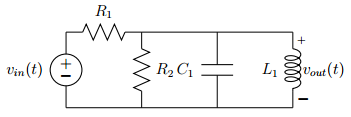
\includegraphics{img/circuito1.png}
				\caption{Circuito 1}	
			\end{figure}			
			Podemos modelar o circuito 1 em relação ao nó após R1. Teríamos a seguinte equação: \\
			\[
				\frac{V_{in} - V_{out}}{R1} - \frac{V_{out}}{R2} - \frac{C\partial V_{out}}{\partial t} - \frac{1}{L} \int V_{out}{\partial t} = 0
			\] 	\\
			Para encontrarmos a E.D.O do circuito, vamos derivar toda esta expressão e separar $V_{out}$ e $V_{in}$, encontrando a seguinte relação:
			\[
				\frac{\partial V_{in}}{\partial t} \left(\frac{1}{R_{1}}\right) = \frac{C \partial^{2} V_{out}}{\partial t^{2}} + \frac{\partial V_{out}}{\partial t} \left(\frac{1}{R_{1}} + \frac{1}{R_{2}} \right) + \frac{V_{out}}{L}
			\] 	\\			
			Em posse da E.D.O, utilizaremos Laplace para encontrar a função de Transferência do Circuito.
			\[
				X(S) \left(\frac{1}{R_{1}}\right) = Y(S)\left(S^{2}C + S \left(\frac{1}{R_{1}} + \frac{1}{R_{2}}\right) + \frac{1}{L} \right) \Rightarrow
			\] 	\\	
			\[
				H(S) = \frac{Y(S)}{X(S)} = \frac{SR_{2}L}{S^{2}\left(R_{1}R_{2}LC\right) + S\left(R_{1}L + R_{2}L\right) + R_{1}R_{2}}
			\] 	\\		
			
			Afim de facilitar os cálculos, tomaremos os seguintes valores para cada elemento do circuito:
			 \begin{itemize}
				\item $R_{1} = 1K \Omega;$
				\item $R_{2} = 10K \Omega;$
				\item $C = 220\mu F;$
				\item $L = 166\eta H;$
			 \end{itemize}		
			 
			Apos aplicar os valores comercias em H(S), temos:
			\[
			H(S) = \frac{100S}{1000S^{2} + 110S + 110}
			\] 	\\					
			
			Utilizando essa função no MatLab para encontrar os polos (quando se zera o denominador), zeros (quando se zera o numerador) e o diagrama de Bode, obtemos o seguintes gráficos:
			
			\begin{figure}[!ht]
				\centering
				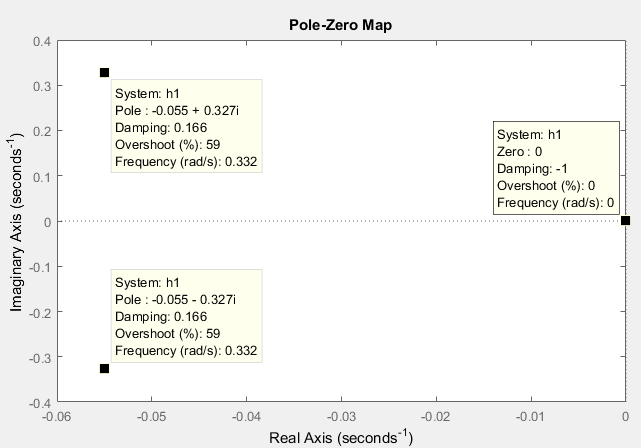
\includegraphics[scale=0.7]{img/1e_circ1.png}
				\caption{Circuito 1 - Polos e Zeros}	
			\end{figure}	
			
			\begin{figure}[!ht]
				\centering
				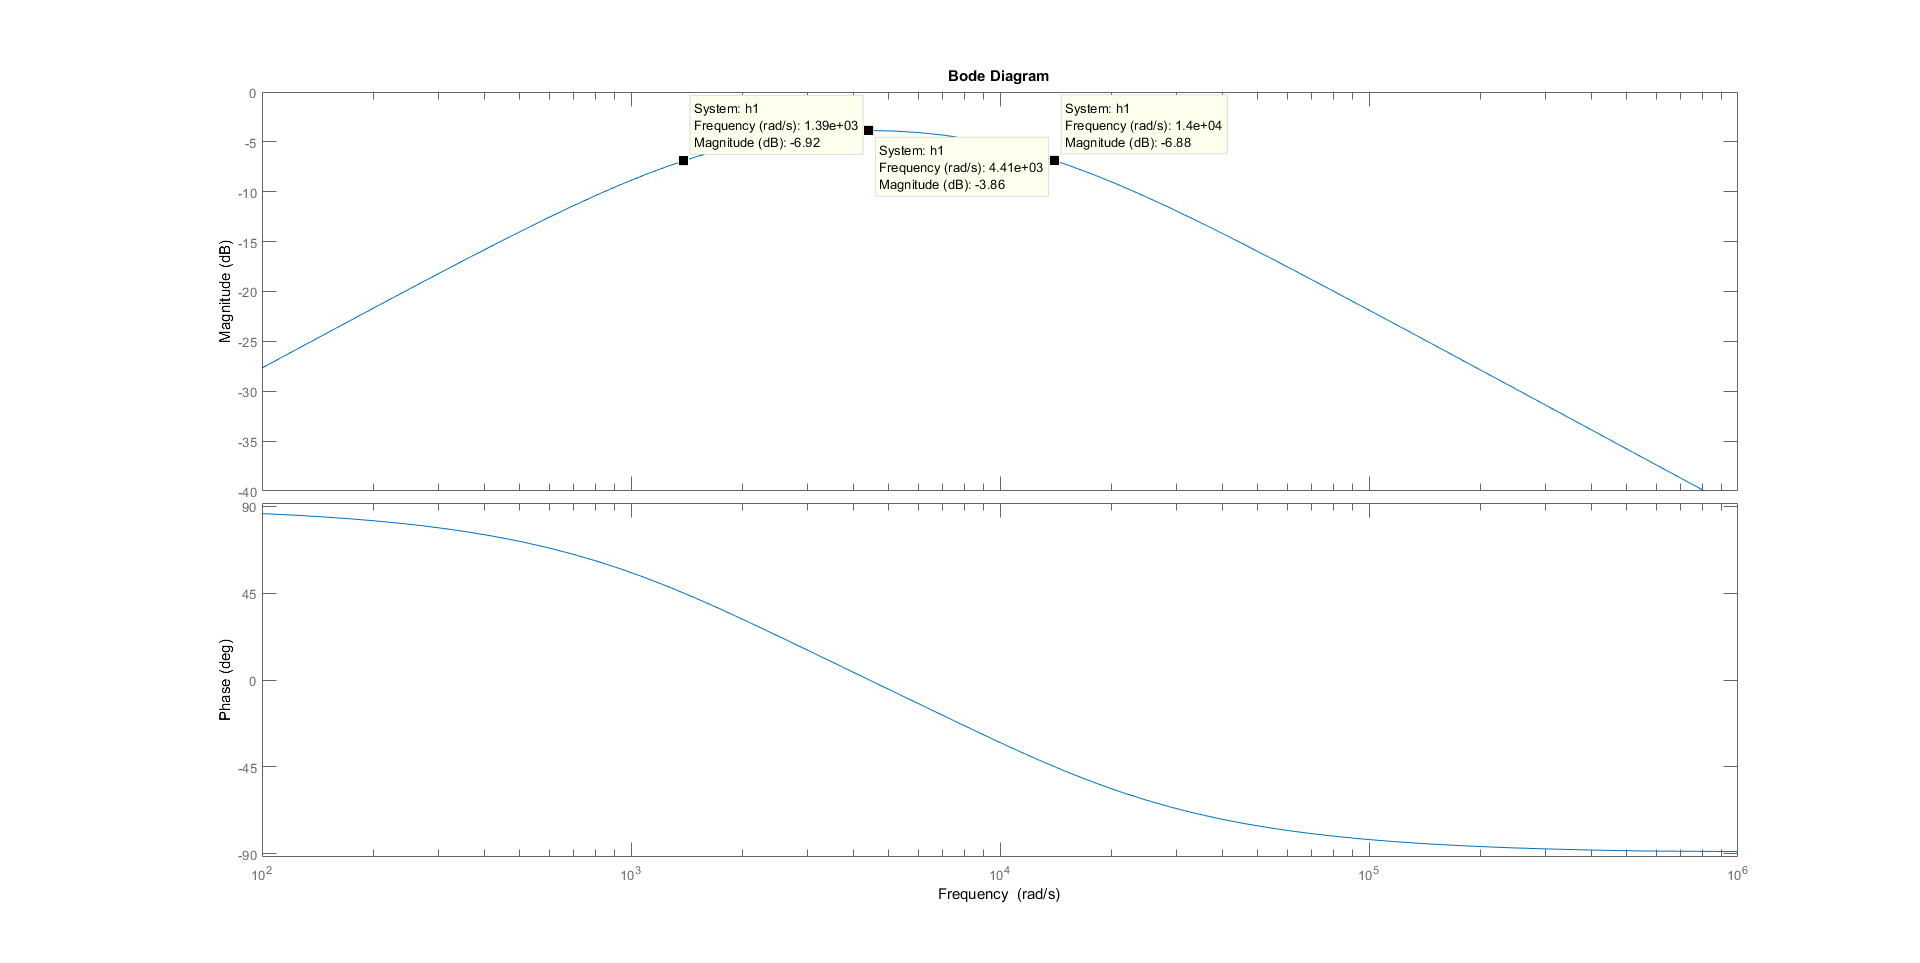
\includegraphics[scale=0.9]{img/1f_circ1.png}
				\caption{Circuito 1 - Diagrama de Bode}	
			\end{figure}						
											
			Analisando-se este circuito, pode-se afirmar que o mesmo é um filtro passa faixa operando na largura de banda de aproximadamente 0.11 rad/sec em um intervalo [0.28, 0.39] rad/sec.
			\newpage
			\subsubsection{Resposta ao degrau unitário}
			\begin{figure}[!ht]
				\centering
				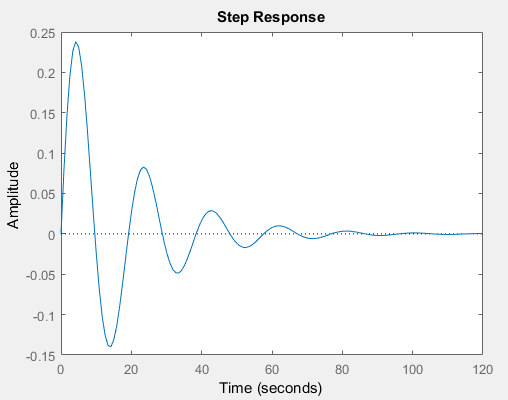
\includegraphics[scale=0.71]{img/1g_circ1.png}
				\caption{Circuito 1 - Resposta ao degrau unitário}	
			\end{figure}					
			\subsubsection{Resposta a rampa unitário}
			\begin{figure}[!ht]
				\centering
				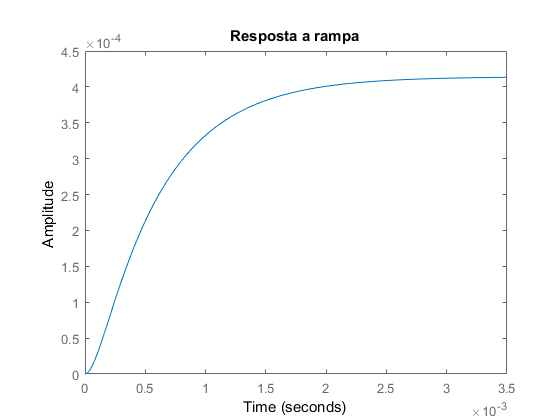
\includegraphics[scale=0.72]{img/1h_circ1.png}
				\caption{Circuito 1 - Resposta a rampa unitária}	
			\end{figure}		

			\subsubsection{Resposta a onda quadrada}
			\begin{figure}[!ht]
				\centering
				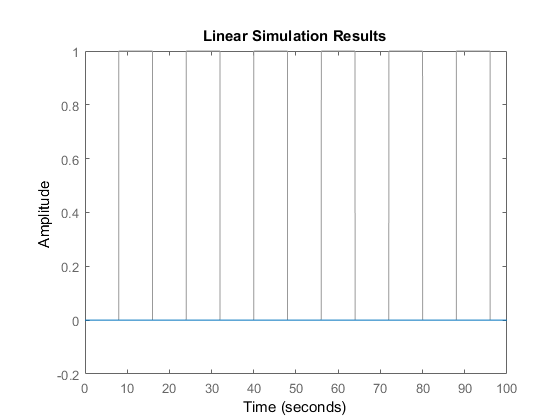
\includegraphics[scale=0.71]{img/1i_circ1.png}
				\caption{Circuito 1 - Resposta a onda quadrada com $\omega = \frac{1}{8}\pi$}	
			\end{figure}			
			\begin{figure}[!ht]
				\centering
				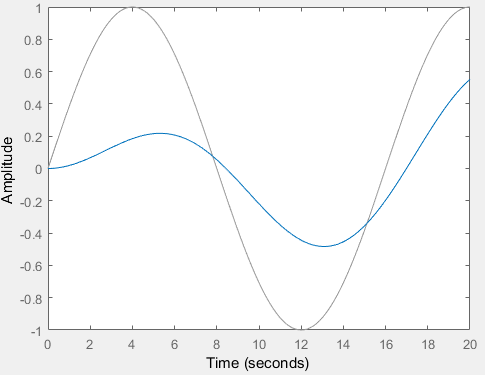
\includegraphics[scale=0.71]{img/1j_circ1.png}
				\caption{Circuito 1 - Resposta ao primeiro harmônico da série de Fourier de um onda quadrada com $\omega = \frac{1}{8}\pi$}	
			\end{figure}		
			\begin{figure}[!ht]
				\centering
				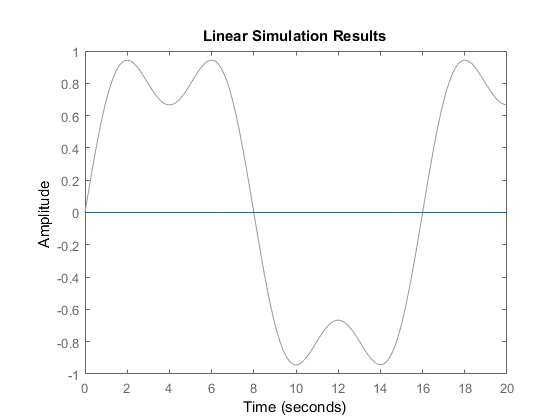
\includegraphics[scale=0.71]{img/1k_circ1.png}
				\caption{Circuito 1 - Resposta ao terceiro harmônico da série de Fourier de um onda quadrada com $\omega = \frac{1}{8}\pi$}	
			\end{figure}			
			\begin{figure}[!ht]
				\centering
				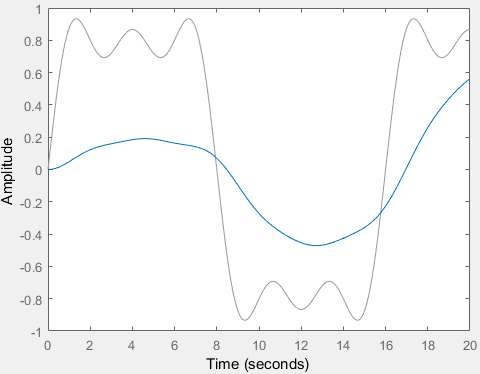
\includegraphics[scale=0.71]{img/1l_circ1.png}
				\caption{Circuito 1 - Resposta ao quinto harmônico da série de Fourier de um onda quadrada com $\omega = \frac{1}{8}\pi$}	
			\end{figure}				
			\begin{figure}[!ht]
				\centering
				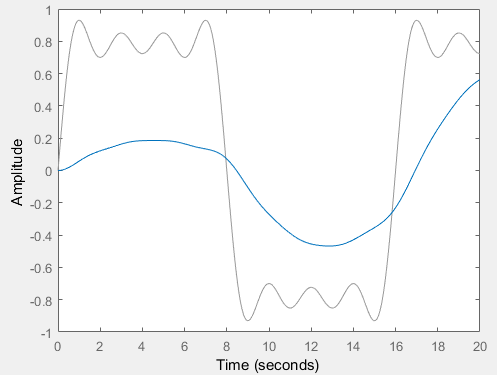
\includegraphics[scale=0.71]{img/1m_circ1.png}
				\caption{Circuito 1 - Resposta ao sétimo harmônico da série de Fourier de um onda quadrada com $\omega = \frac{1}{8}\pi$}	
			\end{figure}
		\newpage
		\subsection{Circuito 2}
			\subsubsection{Determinar a função do circuto}
			\begin{figure}[!hb]
				\centering
				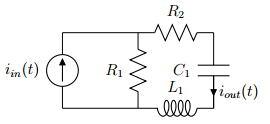
\includegraphics{img/circuito2.png}
				\caption{Circuito 2}	
			\end{figure}			
			
			Para modelarmos utilizaremos as seguintes equações:
			\[				
				 I_{1} = I_{in} - I_{out}
			\] 	\\	
			\[	
				 R_{2}I_{out} + \frac{L \partial I_{out}}{\partial t} - R_{1}I_{1} + \frac{1}{C}\int I_{out}\partial t = 0
			\] 	\\	
			
			Substituindo $I_{1}$ para colocarmos a equação em função de $I_{in}$ e $I_{out}$ e derivando-a para removermos a Integral, temos a E.D.O:
			
			\[	
				\frac{\partial I_{in}}{\partial t}\left(R_{1}\right) = \frac{\partial^{2}I_{out}}{\partial t^{2}}\left(L\right) + \frac{\partial I_{out}}{\partial t}\left(R_{1} + R_{2}\right) + \frac{I_{out}}{C}
			\] 	\\
						
			Transformando essa E.D.O em Laplace, obtemos:
			
			\[	
				X(S)\left(SR_{1}\right) = Y(S)\left(S^{2} + S\left(R_{1} +  R_{2}\right) + \frac{1}{C}\right) \Rightarrow
			\] 	\\			
			\[
			H(S) = \frac{Y(S)}{X(S)} = \frac{S\left(R_{1}C\right)}{S^{2}\left(LC\right) + S\left(R_{1}C + R_{2}C\right) + 1}
			\] 	\\					
			
			Escolhendo os seguintes valores para cada elemento do circuito:
			\begin{itemize}
				\item $R_{1} = 10\Omega;$
				\item $R_{2} = 100\Omega;$
				\item $C = 220\mu F;$
				\item $L = 166\eta H;$
			\end{itemize}	
							
			Encontramos a seguinte função de transferência:
			\[
				H(S) = \frac{10S}{S^{2} + 110S + 1}
			\] 	\\				
			A partir dessa função obtemos os seguintes polos, zeros e diagrama de Bode:
			\begin{figure}[!ht]
				\centering
				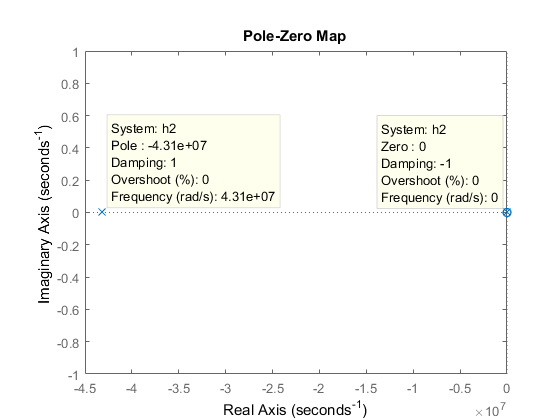
\includegraphics[scale=0.8]{img/1e_circ2.png}
				\caption{Circuito 2 - Polos e Zeros}	
			\end{figure}	

			\begin{figure}[!ht]
				\centering
				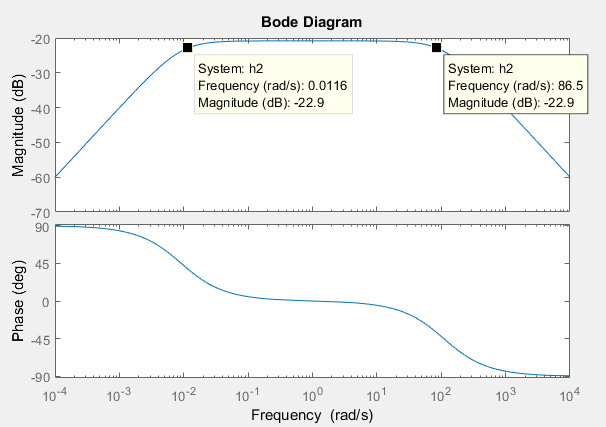
\includegraphics[scale=0.7]{img/1f_circ2.png}
				\caption{Circuito 2 - Diagrama de Bode}	
			\end{figure}			
			\newpage		
			Assim como o circuito da figura 1, temos também um filtro passa faixa que opera nas faixas entre 0.01 rad/seg e 86.5 rad/seg
			
			\subsubsection{Resposta ao degrau unitário}
			\begin{figure}[!ht]
				\centering
				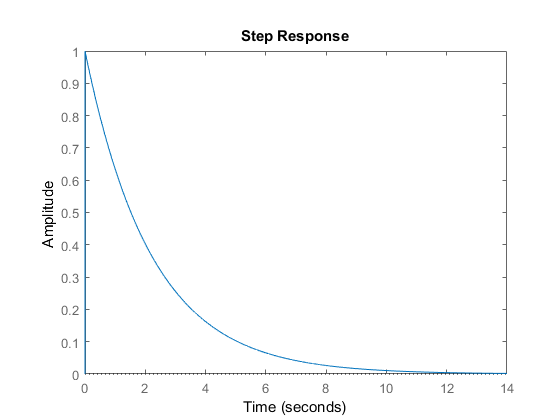
\includegraphics[scale=0.71]{img/1g_circ2.png}
				\caption{Circuito 2 - Resposta ao degrau unitário}	
			\end{figure}					
			\subsubsection{Resposta a rampa unitário}
			\begin{figure}[!ht]
				\centering
				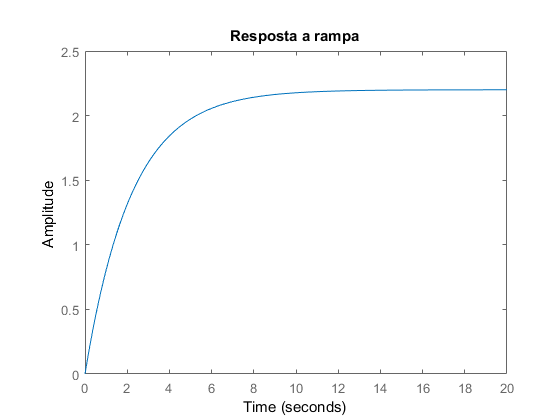
\includegraphics[scale=0.72]{img/1h_circ2.png}
				\caption{Circuito 2 - Resposta a rampa unitária}	
			\end{figure}		
			
			\subsubsection{Resposta a onda quadrada}
			\begin{figure}[!ht]
				\centering
				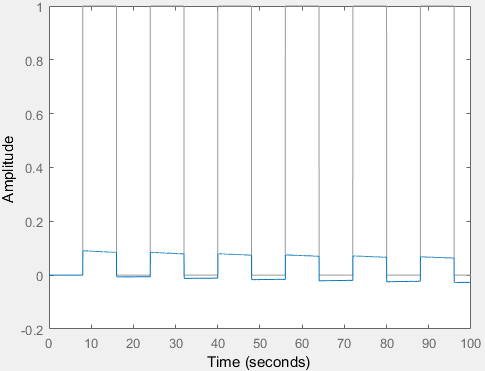
\includegraphics[scale=0.71]{img/1i_circ2.png}
				\caption{Circuito 2 - Resposta a onda quadrada com $\omega = \frac{1}{8}\pi$}	
			\end{figure}			
			\begin{figure}[!ht]
				\centering
				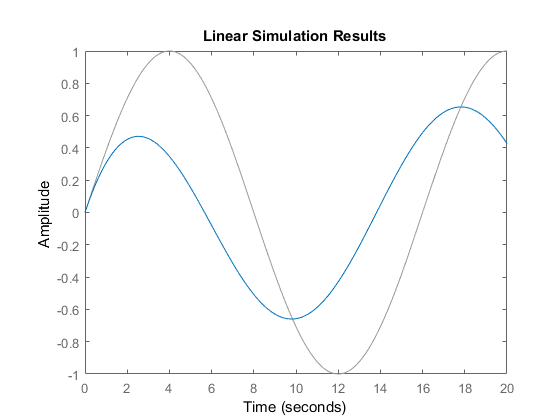
\includegraphics[scale=0.71]{img/1j_circ2.png}
				\caption{Circuito 2 - Resposta ao primeiro harmônico da série de Fourier de um onda quadrada com $\omega = \frac{1}{8}\pi$}	
			\end{figure}		
			\begin{figure}[!ht]
				\centering
				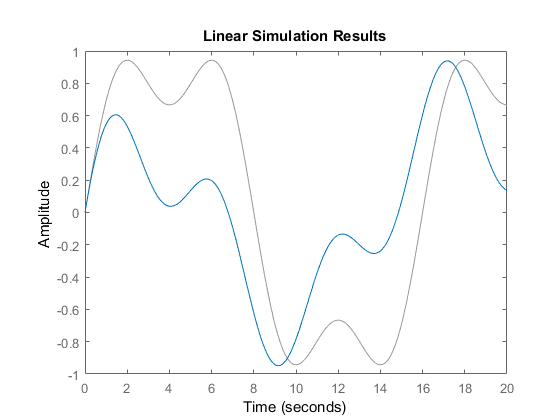
\includegraphics[scale=0.71]{img/1k_circ2.png}
				\caption{Circuito 2 - Resposta ao terceiro harmônico da série de Fourier de um onda quadrada com $\omega = \frac{1}{8}\pi$}	
			\end{figure}			
			\begin{figure}[!ht]
				\centering
				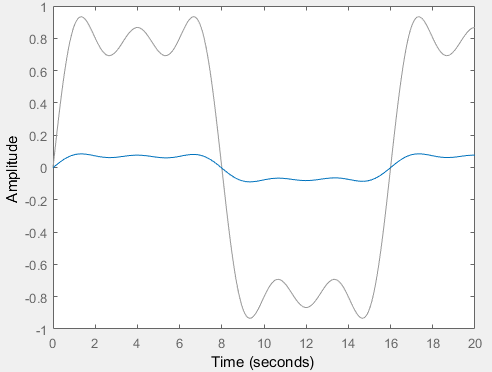
\includegraphics[scale=0.71]{img/1l_circ2.png}
				\caption{Circuito 2 - Resposta ao quinto harmônico da série de Fourier de um onda quadrada com $\omega = \frac{1}{8}\pi$}	
			\end{figure}		
		    \clearpage
			\begin{figure}[!ht]
				\centering
				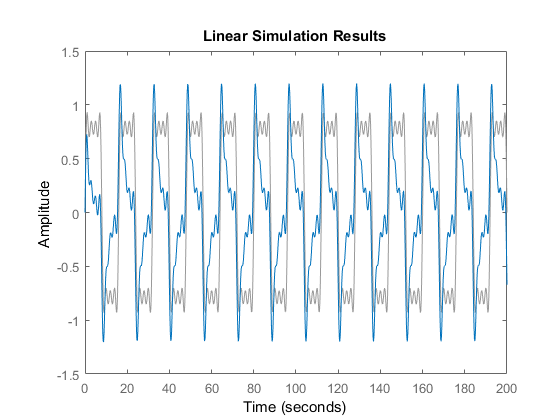
\includegraphics[scale=0.71]{img/1m_circ2.png}
				\caption{Circuito 2 - Resposta ao sétimo harmônico da série de Fourier de um onda quadrada com $\omega = \frac{1}{8}\pi$}	
			\end{figure}			
		\subsection{Circuito 3}
			\subsubsection{Determinar a função do circuto}
			\begin{figure}[!ht]
				\centering
				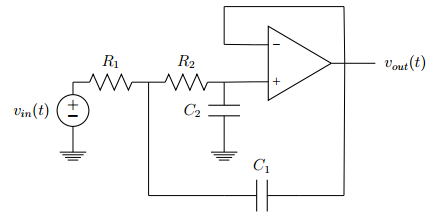
\includegraphics{img/circuito3.png}
				\caption{Circuito 3}	
			\end{figure}			
			
			Este circuito, também conhecido como topologia de Sallen-Key, sabendo que o AmpOp possui impedância infinita em sua entrada, que $V^{-} = V^{+}$, que $V^{-} = V_{out}$ e chamando $V_{a}$ da tensão que passa por $C_{1}$, obtemos:
				
			\[
			V_{a} = V_{out} + R_{2}C_{2}\frac{\partial V_{out}}{\partial t}
			\] 	\\					
			
			Utilizando a lei dos nós entre $R_{1}$ e $R_{2}$ e já substituindo $V_{a}$ por $V_{out}$ temos:
			
			\[
			\frac{V_{in}}{R_{1}} = R_{2}C_{1}C_{2}\frac{\partial^{2} V_{out}}{\partial t^{2}} + \left(C_{2} + \frac{R_{2}C_{2}}{R_{1}}\right)\frac{\partial V_{out}}{\partial t} +  \frac{V_{out}}{R_{1}}
			\] 	\\			
			
			Com esta E.D.O, podemos encontrar a seguinte função de transferência utilizando o mesmo método empregado nos circuitos anteriores, com isso temos:
			
			\[
			H(S) = \frac{1}{S^{2}\left(R_{1}R_{2}C_{1}C_{2}\right) + S\left(R_{1}C_{2} + R_{2}C_{2}\right) + 1}
			\] 	\\					
			
			Utilizando os valores para cada elemento do circuito:
			\begin{itemize}
				\item $R_{1} = 10\Omega;$
				\item $R_{2} = 100\Omega;$
				\item $C_{1} = 2F;$
				\item $C_{2} = 1F;$
			\end{itemize}				

			Encontramos a seguinte função de transferência:
			\[
			H(S) = \frac{1}{2000S^{2} + 110S + 1}
			\] 	\\				
			
			Que nos gera os seguintes polos, zeros e diagrama de Bode:	
			\begin{figure}[!ht]
				\centering
				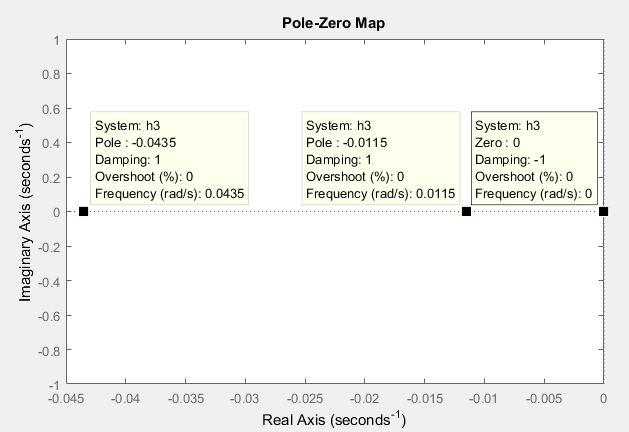
\includegraphics[scale=0.7]{img/1e_circ3.png}
				\caption{Circuito 3 - Polos e Zeros}	
			\end{figure}	
			\newpage
			\begin{figure}[!ht]
				\centering
				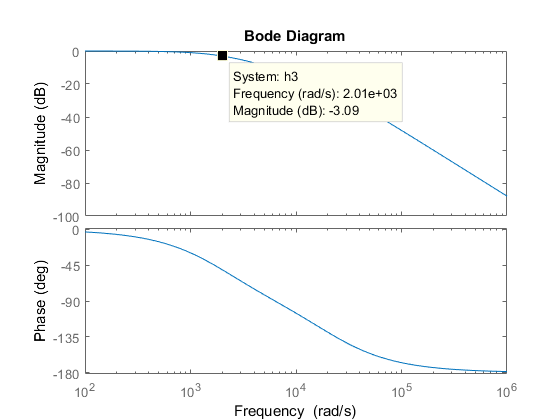
\includegraphics[scale=0.7]{img/1f_circ3.png}
				\caption{Circuito 3 - Diagrama de Bode}	
			\end{figure}			
			Pela a analise do diagrama de Bode, pode-se afirmar que esse circuito é um filtro passa alta com frequência no seu menor polo de 0.01 rad/sec.
			\subsubsection{Resposta ao degrau unitário}
			\begin{figure}[!ht]
				\centering
				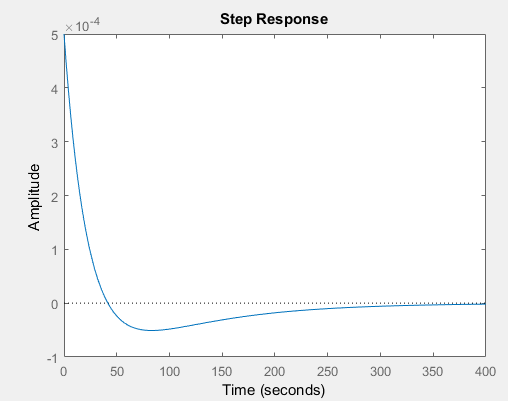
\includegraphics[scale=0.71]{img/1g_circ3.png}
				\caption{Circuito 3 - Resposta ao degrau unitário}	
			\end{figure}					
			\subsubsection{Resposta a rampa unitário}
			\begin{figure}[!ht]
				\centering
				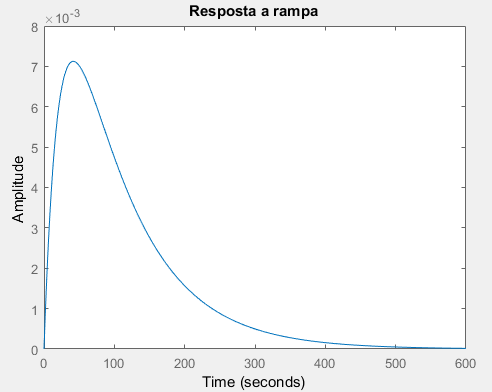
\includegraphics[scale=0.72]{img/1h_circ3.png}
				\caption{Circuito 3 - Resposta a rampa unitária}	
			\end{figure}		
			
			\subsubsection{Resposta a onda quadrada}
			\begin{figure}[!ht]
				\centering
				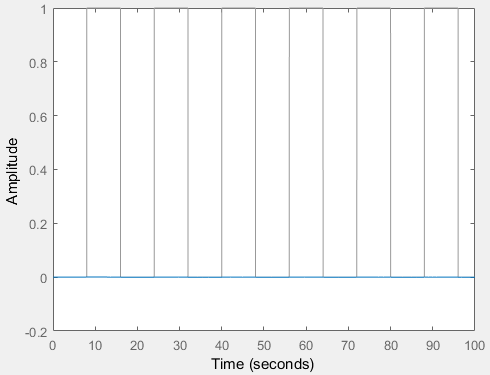
\includegraphics[scale=0.71]{img/1i_circ3.png}
				\caption{Circuito 3 - Resposta a onda quadrada com $\omega = \frac{1}{8}\pi$}	
			\end{figure}			
			\begin{figure}[!ht]
				\centering
				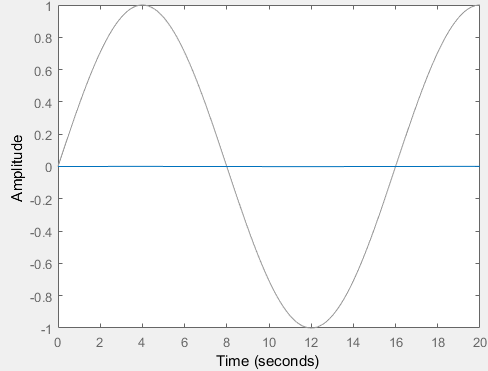
\includegraphics[scale=0.71]{img/1j_circ3.png}
				\caption{Circuito 3 - Resposta ao primeiro harmônico da série de Fourier de um onda quadrada com $\omega = \frac{1}{8}\pi$}	
			\end{figure}		
			\begin{figure}[!ht]
				\centering
				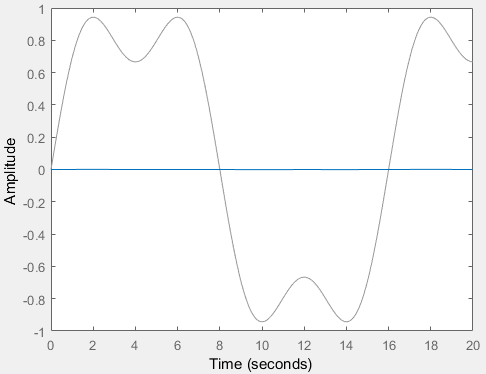
\includegraphics[scale=0.71]{img/1k_circ3.png}
				\caption{Circuito 3 - Resposta ao terceiro harmônico da série de Fourier de um onda quadrada com $\omega = \frac{1}{8}\pi$}	
			\end{figure}			
			\begin{figure}[!ht]
				\centering
				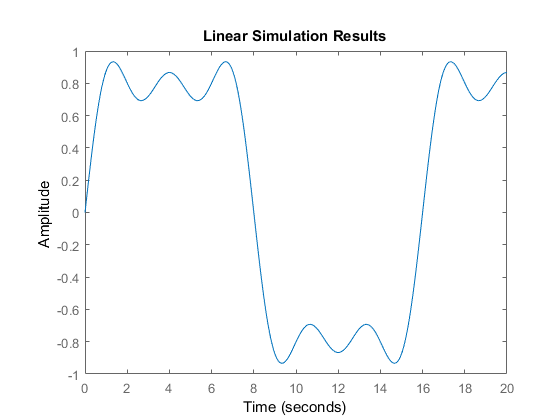
\includegraphics[scale=0.71]{img/1l_circ3.png}
				\caption{Circuito 3 - Resposta ao quinto harmônico da série de Fourier de um onda quadrada com $\omega = \frac{1}{8}\pi$}	
			\end{figure}		
			\clearpage
			\begin{figure}[!ht]
				\centering
				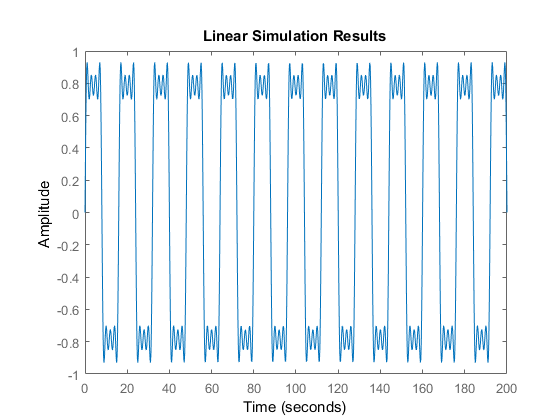
\includegraphics[scale=0.71]{img/1m_circ3.png}
				\caption{Circuito 3 - Resposta ao sétimo harmônico da série de Fourier de um onda quadrada com $\omega = \frac{1}{8}\pi$}	
			\end{figure}				
		\subsection{Circuito 4}
			\subsubsection{Determinar a função do circuto}
			\begin{figure}[!ht]
				\centering
				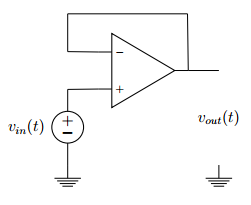
\includegraphics{img/circuito4.png}
				\caption{Circuito 4}	
			\end{figure}		
			
			Esse circuito, conhecido como buffer, é utilizado como um isolador. Como $V_{in}$ é igual a $V_{out}$, sua função de transferência  H(S) = 1. Não existem polos nem zeros para esse circuito e seu diagrama de Bode permanece em 0.
			\begin{figure}[!ht]
				\centering
				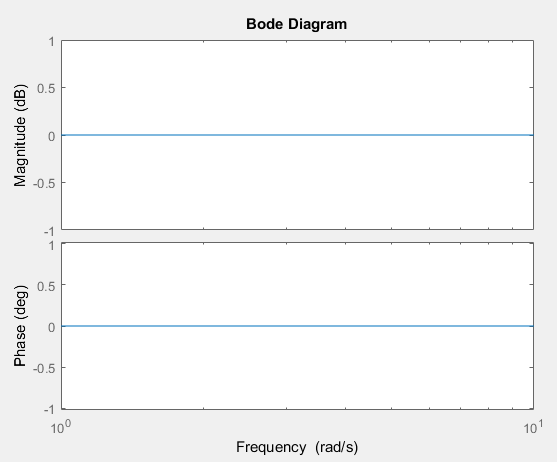
\includegraphics[scale=0.7]{img/1f_circ4.png}
				\caption{Circuito 4 - Diagrama de Bode}	
			\end{figure}	
			\subsubsection{Resposta ao degrau unitário}
			\begin{figure}[!ht]
				\centering
				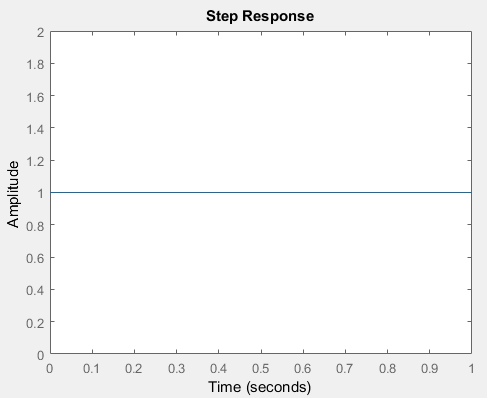
\includegraphics[scale=0.71]{img/1g_circ4.png}
				\caption{Circuito 4 - Resposta ao degrau unitário}	
			\end{figure}					
			\subsubsection{Resposta a rampa unitário}
			\begin{figure}[!ht]
				\centering
				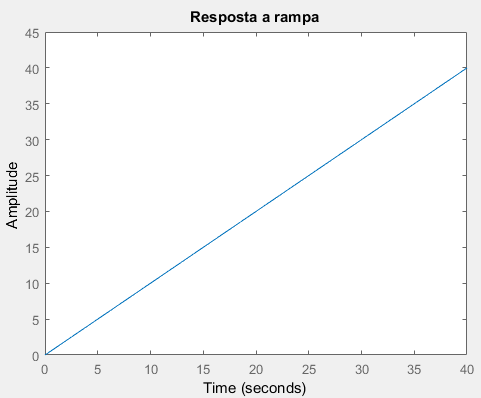
\includegraphics[scale=0.72]{img/1h_circ4.png}
				\caption{Circuito 4 - Resposta a rampa unitária}	
			\end{figure}		
			
			\subsubsection{Resposta a onda quadrada}
			\begin{figure}[!ht]
				\centering
				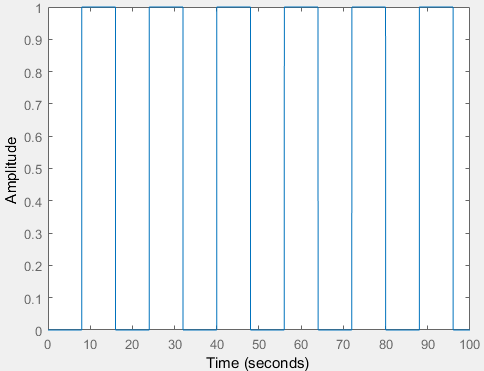
\includegraphics[scale=0.71]{img/1i_circ4.png}
				\caption{Circuito 4 - Resposta a onda quadrada com $\omega = \frac{1}{8}\pi$}	
			\end{figure}			
			\begin{figure}[!ht]
				\centering
				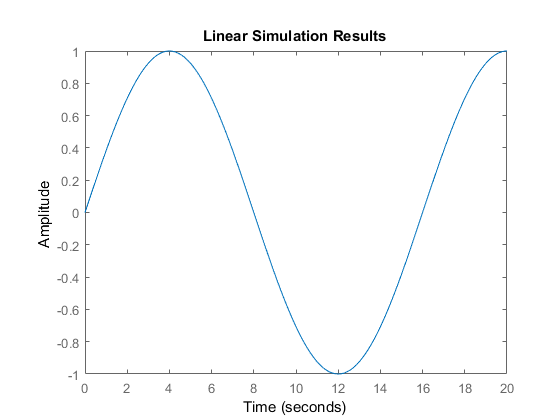
\includegraphics[scale=0.71]{img/1j_circ4.png}
				\caption{Circuito 4 - Resposta ao primeiro harmônico da série de Fourier de um onda quadrada com $\omega = \frac{1}{8}\pi$}	
			\end{figure}		
			\begin{figure}[!ht]
				\centering
				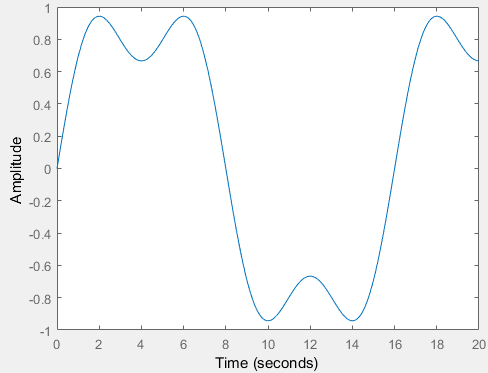
\includegraphics[scale=0.71]{img/1k_circ4.png}
				\caption{Circuito 4 - Resposta ao terceiro harmônico da série de Fourier de um onda quadrada com $\omega = \frac{1}{8}\pi$}	
			\end{figure}			
			\begin{figure}[!ht]
				\centering
				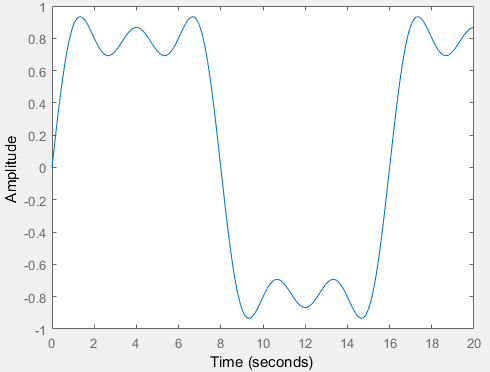
\includegraphics[scale=0.71]{img/1l_circ4.png}
				\caption{Circuito 4 - Resposta ao quinto harmônico da série de Fourier de um onda quadrada com $\omega = \frac{1}{8}\pi$}	
			\end{figure}		
			\begin{figure}[!ht]
				\centering
				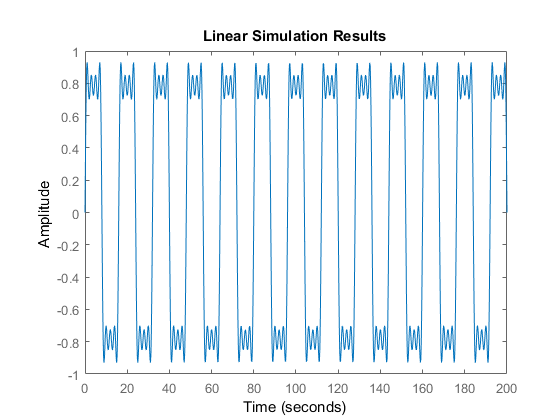
\includegraphics[scale=0.71]{img/1m_circ4.png}
				\caption{Circuito 4 - Resposta ao sétimo harmônico da série de Fourier de um onda quadrada com $\omega = \frac{1}{8}\pi$}	
			\end{figure}					
		\clearpage		
		\subsection{Circuito 5}
			\subsubsection{Determinar a função do circuto}
			\begin{figure}[!ht]
				\centering
				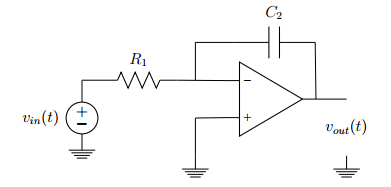
\includegraphics{img/circuito5.png}
				\caption{Circuito 5}	
			\end{figure}		
			
			Esse circuito pode ser escrito  como:
			\[
			\frac{V_{in}}{R} + C\frac{\partial V_{out}}{\partial t} = 0
			\] 	\\			
			
			Transformando esta E.D.O com Laplace utilizando o mesmo método dos circuitos passados, obtemos:
			
			\[
			H(S) = \frac{-1}{RCS}
			\] 	\\				
			
			Tomando os seguintes valores para os elementos do circuito:
			\begin{itemize}
				\item $R = 10\Omega;$
				\item $C = 1F;$
			\end{itemize}		
			
			Temos a seguinte equação de transferência:	
			
			\[
			H(S) = \frac{-1}{10S}
			\] 	\\					
			
			A partir dessa equação, obtemos os seguintes polos, zeros e diagrama de Bode:	
			
			\begin{figure}[!ht]
				\centering
				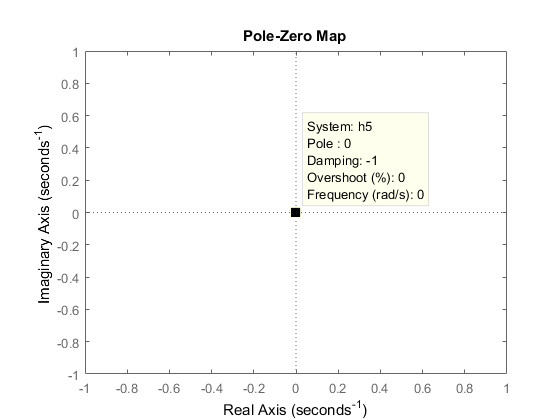
\includegraphics[scale=0.75]{img/1e_circ5.png}
				\caption{Circuito 5 - Polos e Zeros}	
			\end{figure}	
			\newpage
			\begin{figure}[!ht]
				\centering
				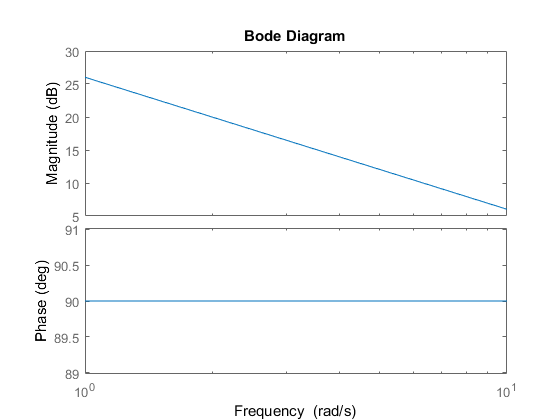
\includegraphics[scale=0.78]{img/1f_circ5.png}
				\caption{Circuito 5 - Diagrama de Bode}	
			\end{figure}				
			
			Este circuito corresponde a um filtro passa baixa integrador de apenas um polo.	
			
			\subsubsection{Resposta ao degrau unitário}
			\begin{figure}[!ht]
				\centering
				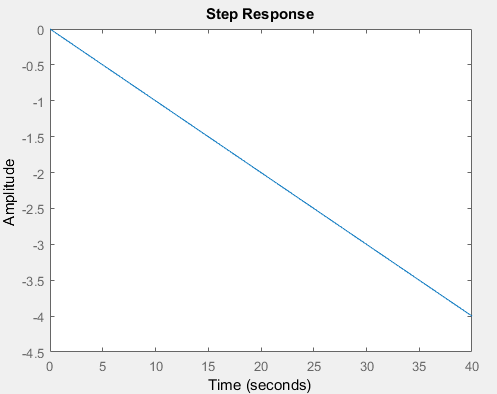
\includegraphics[scale=0.71]{img/1g_circ5.png}
				\caption{Circuito 5 - Resposta ao degrau unitário}	
			\end{figure}					
			\subsubsection{Resposta a rampa unitária}
			\begin{figure}[!ht]
				\centering
				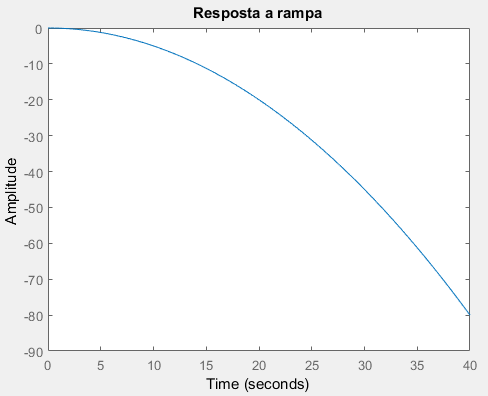
\includegraphics[scale=0.72]{img/1h_circ5.png}
				\caption{Circuito 5 - Resposta a rampa unitária}	
			\end{figure}		
			
			\subsubsection{Resposta a onda quadrada}
			\begin{figure}[!ht]
				\centering
				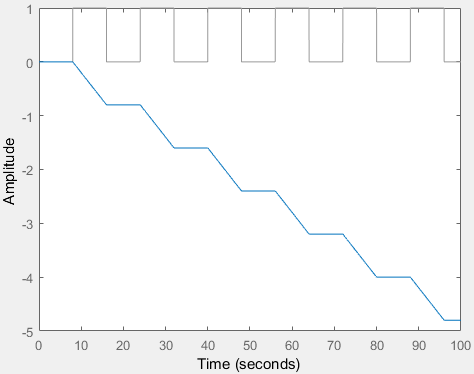
\includegraphics[scale=0.71]{img/1i_circ5.png}
				\caption{Circuito 5 - Resposta a onda quadrada com $\omega = \frac{1}{8}\pi$}	
			\end{figure}			
			\begin{figure}[!ht]
				\centering
				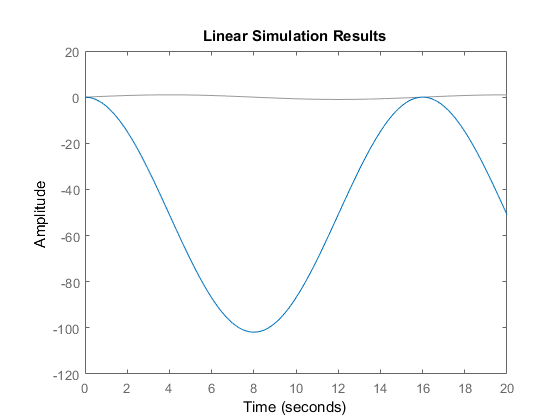
\includegraphics[scale=0.71]{img/1j_circ5.png}
				\caption{Circuito 5 - Resposta ao primeiro harmônico da série de Fourier de um onda quadrada com $\omega = \frac{1}{8}\pi$}	
			\end{figure}		
			\begin{figure}[!ht]
				\centering
				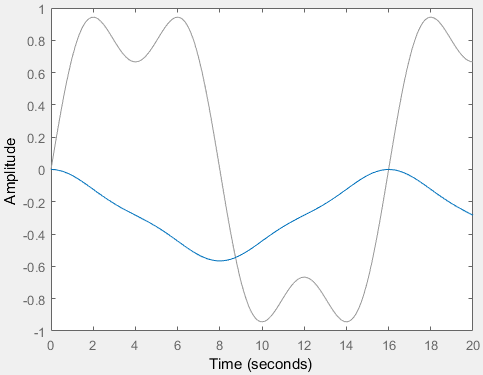
\includegraphics[scale=0.71]{img/1k_circ5.png}
				\caption{Circuito 5 - Resposta ao terceiro harmônico da série de Fourier de um onda quadrada com $\omega = \frac{1}{8}\pi$}	
			\end{figure}			
			\begin{figure}[!ht]
				\centering
				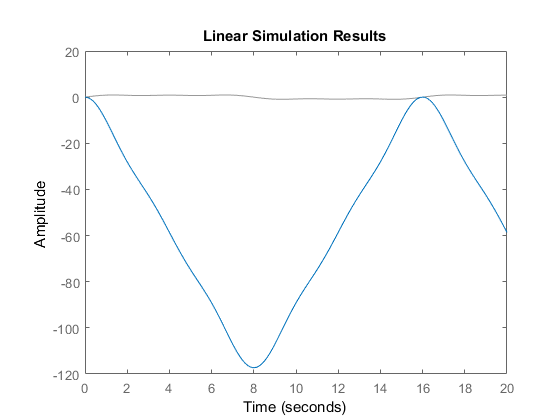
\includegraphics[scale=0.71]{img/1l_circ5.png}
				\caption{Circuito 5 - Resposta ao quinto harmônico da série de Fourier de um onda quadrada com $\omega = \frac{1}{8}\pi$}	
			\end{figure}		
			\begin{figure}[!ht]
				\centering
				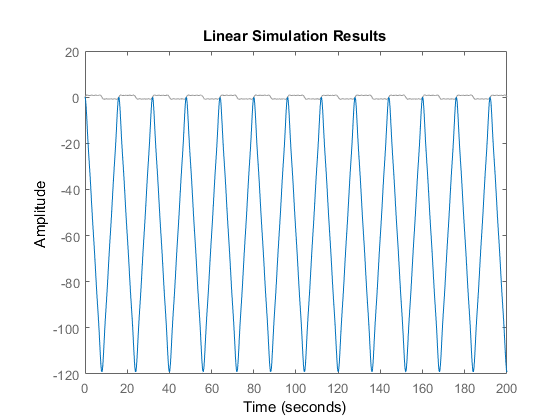
\includegraphics[scale=0.71]{img/1m_circ5.png}
				\caption{Circuito 5 - Resposta ao sétimo harmônico da série de Fourier de um onda quadrada com $\omega = \frac{1}{8}\pi$}	
			\end{figure}						
									
	\clearpage
	\section{Quest\~{a}o 2}
	
	\begin{figure}[!ht]
		\centering
		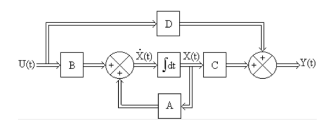
\includegraphics{img/db.png}
		\caption{Diagrama de Blocos}	
	\end{figure}	
	\subsection{Equações do diagrama}
	Seguindo as regras definidas no trabalho em relação aos valores de A, B, C e D para o diagrama de blocos, temos:
		\begin{itemize}
			\item a = -22;
			\item b = 7;
			\item c = 3;
			\item d = 4;
		\end{itemize}		
		
	Pare que o circuito possua estabilidade BIBO, precisamos que o valor de A seja negativo, caso contrario, o circuito é instável.
	
	Com esses valores obtemos as seguintes equações para o diagrama de blocos abaixo:
	
		\begin{itemize}
			\item y(t) = 4u(t) + 3x(t) \textit{(Item (e) da questão 2)};
			\item B = 7u(t);
			\item C = 3x(t);
			\item D = 4u(t);
			\item $x^{'}(t) = 7u(t) - 22x(t)$ \textit{(Item (d) da questão 2)};
		\end{itemize}	
		
	Sabendo que $x(t) = \frac{y(t) - 4u(t)}{3}$ e  $x^{'} = \frac{y^{'}(t) - 4u^{'}(t)}{3}$, obtemos a seguinte E.D.O:
	
	\[
	\frac{\partial y(t)}{\partial t} + 22y(t) = 4\frac{\partial y(t)}{\partial t} + 109u(t)
	\] 	\\	
	
	Aplicando Laplace, obtemos a seguinte função de transferência:
	
	\[
	H(S) = \frac{Y(S)}{U(S)} = \frac{4S + 109}{S +22}
	\] 	\\		

	De posse da função de transferência, podemos encontrar os seguintes polos e zeros e o diagrama de Bode:
	\begin{figure}[!ht]
		\centering
		\includegraphics{img/2b.png}
		\caption{Polos e Zeros}	
	\end{figure}	
	\begin{figure}[!ht]
		\includegraphics{img/2c.png}
		\caption{Diagrama de Bode}	
	\end{figure}			
	\newpage
	\clearpage
	\subsection{Resposta ao degrau unitário}
		\begin{figure}[!ht]
			\centering
			\includegraphics[scale=0.71]{img/2f.png}
			\caption{Resposta ao degrau unitário}	
		\end{figure}		
	
	\subsection{Resposta a rampa unitária}
		\begin{figure}[!ht]
			\centering
			\includegraphics[scale=0.71]{img/2g.png}
			\caption{Resposta a rampa unitária}	
		\end{figure}				

			\subsection{Resposta a onda quadrada}
			\begin{figure}[!ht]
				\centering
				\includegraphics[scale=0.71]{img/2h.png}
				\caption{Resposta a onda quadrada com $\omega = \frac{1}{4}\pi$}	
			\end{figure}			
			\begin{figure}[!ht]
				\centering
				\includegraphics[scale=0.71]{img/2i.png}
				\caption{Resposta ao primeiro harmônico da série de Fourier de um onda quadrada com $\omega = \frac{1}{2}\pi$}	
			\end{figure}		
			\begin{figure}[!ht]
				\centering
				\includegraphics[scale=0.71]{img/2j.png}
				\caption{Resposta ao terceiro harmônico da série de Fourier de um onda quadrada com $\omega = \frac{1}{2}\pi$}	
			\end{figure}			
			\begin{figure}[!ht]
				\centering
				\includegraphics[scale=0.71]{img/2k.png}
				\caption{Resposta ao quinto harmônico da série de Fourier de um onda quadrada com $\omega = \frac{1}{2}\pi$}	
			\end{figure}		
			\begin{figure}[!ht]
				\centering
				\includegraphics[scale=0.71]{img/2l.png}
				\caption{Resposta ao sétimo harmônico da série de Fourier de um onda quadrada com $\omega = \frac{1}{2}\pi$}	
			\end{figure}		
			\clearpage
							
	\section{Quest\~{a}o 3}
		Resolva as questões para os sistemas descritos pelas seguintes funções de transferência:
		\[
		H(S)= \frac{1 + \alpha S}{S^{2} + 2S +  2}
		\] 	\\			
		\[
		H(S)= \frac{S + 10^{4}}{S^{2} + 2\beta S +  100}
		\] 	\\				
		
		\subsection{E.D.O dos sistemas}

			\subsubsection{Sistema 1}
				\[
				X(S)[1+ \alpha S] = Y(S)[S^{2} + 2S + 2] \Rightarrow
				\] 	\\			
				\[						
				\alpha \frac{\partial x(t)}{\partial t} + x(t) = \frac{\partial^{2}y(t)}{\partial^{2}t} + 2\frac{\partial^y(t)}{\partial t} + 2y(t)
				\] 	\\				
			\subsubsection{Sistema 2}
				\[
				X(S)[S + 10^{4}] = Y(S)[S^{2} + 2\beta S +  100] \Rightarrow
				\] 	\\			
				\[						
				\frac{\partial x(t)}{\partial t} + 10^{4}x(t) = \frac{\partial^{2}y(t)}{\partial^{2}t} + 2 \beta\frac{\partial y(t)}{\partial t} + 100y(t)
				\] 	\\				
				\newpage
		\subsection{Polos e zeros}	
			\subsubsection{Variando em $\alpha$}
			\begin{figure}[!ht]
				\centering
				\includegraphics[scale=0.5]{img/3b_alfa.png}
				\caption{Polos e Zeros variando em $\alpha$}	
			\end{figure}				
			\subsubsection{Variando em $\beta$}		
			\begin{figure}[!ht]
				\centering
				\includegraphics[scale=0.55]{img/3b_beta.png}
				\caption{Polos e Zeros variando em $\beta$}	
			\end{figure}					
		\subsection{Diagrama de Bode}		
			\subsubsection{Variando em $\alpha$}
			\begin{figure}[!ht]
				\centering
				\includegraphics[scale=0.42]{img/3c_alfa.png}
				\caption{Diagrama de Bode variando em $\alpha$}	
			\end{figure}				
			\subsubsection{Variando em $\beta$}	
			\begin{figure}[!ht]
				\centering
				\includegraphics[scale=0.46]{img/3c_beta.png}
				\caption{Diagrama de Bode variando em $\beta$}	
			\end{figure}			
		\subsection{Resposta ao Degrau Unitário}		
			\subsubsection{Variando em $\alpha$}
			\begin{figure}[!ht]
				\centering
				\includegraphics[scale=0.45]{img/3d_alfa.png}
				\caption{Resposta ao Degrau Unitário variando em $\alpha$}	
			\end{figure}				
			\subsubsection{Variando em $\beta$}
			\begin{figure}[!ht]
				\centering
				\includegraphics[scale=0.5]{img/3d_beta.png}
				\caption{Resposta ao Degrau Unitário variando em $\beta$}	
			\end{figure}	
    	\newpage				
		\subsection{Resposta a Rampa Unitária}		
		\subsubsection{Variando em $\alpha$}
		\begin{figure}[!ht]
			\centering
			\includegraphics[scale=0.5]{img/3e_alfa.png}
			\caption{Resposta a rampa Unitária variando em $\alpha$}	
		\end{figure}				
		\subsubsection{Variando em $\beta$}
		\begin{figure}[!ht]
			\centering
			\includegraphics[scale=0.45]{img/3e_beta.png}
			\caption{Resposta a rampa Unitária variando em $\beta$}	
		\end{figure}
		\subsection{Resposta a onda quadrada}					
			\subsubsection{Variando em $\alpha$}
			\begin{figure}[!ht]
				\centering
				\includegraphics[scale=0.4]{img/3f_alfa.png}
				\caption{Resposta a onda quadrada com $\omega = \frac{1}{8}\pi$}	
			\end{figure}			
			\begin{figure}[!ht]
				\centering
				\includegraphics[scale=0.5]{img/3g_alfa.png}
				\caption{Resposta ao primeiro harmônico da série de Fourier de um onda quadrada com $\omega = \frac{1}{4}\pi$}	
			\end{figure}		
			\begin{figure}[!ht]
				\centering
				\includegraphics[scale=0.5]{img/3h_alfa.png}
				\caption{Resposta ao terceiro harmônico da série de Fourier de um onda quadrada com $\omega = \frac{1}{4}\pi$}	
			\end{figure}			
			\begin{figure}[!ht]
				\centering
				\includegraphics[scale=0.5]{img/3i_alfa.png}
				\caption{Resposta ao quinto harmônico da série de Fourier de um onda quadrada com $\omega = \frac{1}{4}\pi$}	
			\end{figure}		
			\begin{figure}[!ht]
				\centering
				\includegraphics[scale=0.57]{img/3j_alfa.png}
				\caption{Resposta ao sétimo harmônico da série de Fourier de um onda quadrada com $\omega = \frac{1}{4}\pi$}	
			\end{figure}	
			\clearpage		
			\subsubsection{Variando em $\beta$}
			\begin{figure}[!ht]
				\centering
				\includegraphics[scale=0.46]{img/3f_beta.png}
				\caption{Resposta a onda quadrada com $\omega = \frac{1}{8}\pi$}	
			\end{figure}			
			\begin{figure}[!ht]
				\centering
				\includegraphics[scale=0.57]{img/3g_beta.png}
				\caption{Resposta ao primeiro harmônico da série de Fourier de um onda quadrada com $\omega = \frac{1}{4}\pi$}	
			\end{figure}		
			\begin{figure}[!ht]
				\centering
				\includegraphics[scale=0.52]{img/3h_beta.png}
				\caption{Resposta ao terceiro harmônico da série de Fourier de um onda quadrada com $\omega = \frac{1}{4}\pi$}	
			\end{figure}			
			\begin{figure}[!ht]
				\centering
				\includegraphics[scale=0.48]{img/3i_beta.png}
				\caption{Resposta ao quinto harmônico da série de Fourier de um onda quadrada com $\omega = \frac{1}{4}\pi$}	
			\end{figure}		
			\begin{figure}[!ht]
				\centering
				\includegraphics[scale=0.5]{img/3j_beta.png}
				\caption{Resposta ao sétimo harmônico da série de Fourier de um onda quadrada com $\omega = \frac{1}{4}\pi$}	
			\end{figure}					
	
	\subsection{Resposta a cossenoides}	
	\subsubsection{Variando frequências nos valores de $\alpha$}	
			\begin{figure}[!ht]
				\centering
				\includegraphics[scale=0.45]{img/3k_alfa1.png}
				\caption{Resposta para $\alpha$ = 0.001 em frequências variantes}	
			\end{figure}		
			\begin{figure}[!ht]
				\centering
				\includegraphics[scale=0.48]{img/3k_alfa2.png}
				\caption{Resposta para $\alpha$ = 0.01 em frequências variantes}	
			\end{figure}			
			\begin{figure}[!ht]
				\centering
				\includegraphics[scale=0.48]{img/3k_alfa3.png}
				\caption{Resposta para $\alpha$ = 0.1 em frequências variantes}	
			\end{figure}				
			\begin{figure}[!ht]
				\centering
				\includegraphics[scale=0.52]{img/3k_alfa4.png}
				\caption{Resposta para $\alpha$ = 1 em frequências variantes}	
			\end{figure}		
			\begin{figure}[!ht]
				\centering
				\includegraphics[scale=0.52]{img/3k_alfa5.png}
				\caption{Resposta para $\alpha$ = 10 em frequências variantes}	
			\end{figure}		
			\begin{figure}[!ht]
				\centering
				\includegraphics[scale=0.48]{img/3k_alfa6.png}
				\caption{Resposta para $\alpha$ = 100 em frequências variantes}	
			\end{figure}		
			\begin{figure}[!ht]
				\centering
				\includegraphics[scale=0.49]{img/3k_alfa7.png}
				\caption{Resposta para $\alpha$ = 1000 em frequências variantes}	
			\end{figure}				
			\clearpage							
	\subsubsection{Variando frequências nos valores de $\beta$}
			\begin{figure}[!ht]
				\centering
				\includegraphics[scale=0.58]{img/3k_beta1.png}
				\caption{Resposta para $\beta$ = 0.001 em frequências variantes}	
			\end{figure}		
			\begin{figure}[!ht]
				\centering
				\includegraphics[scale=0.53]{img/3k_beta2.png}
				\caption{Resposta para $\beta$ = 0.01 em frequências variantes}	
			\end{figure}			
			\begin{figure}[!ht]
				\centering
				\includegraphics[scale=0.49]{img/3k_beta3.png}
				\caption{Resposta para $\beta$ = 0.1 em frequências variantes}	
			\end{figure}				
			\begin{figure}[!ht]
				\centering
				\includegraphics[scale=0.57]{img/3k_beta4.png}
				\caption{Resposta para $\beta$ = 1 em frequências variantes}	
			\end{figure}		
			\begin{figure}[!ht]
				\centering
				\includegraphics[scale=0.57]{img/3k_beta5.png}
				\caption{Resposta para $\beta$ = 10 em frequências variantes}	
			\end{figure}

	\section{Conclusão}
		
	O Trabalho é muito importante para o aprendizado, ele trás a pratica para alguns temas muito abstratos falados durante a aula. A compreensão pratica do problema nos mostra a real utilidade da matéria.
	
	Embora a parte de analise de circuito seja algo extra que só sera aprendido profundamente na matéria de Circuitos Elétricos, com dependência curricular de Sistemas Lineares I, os circuitos mostrados são de fácil modelagem. Em relação ao diagrama de blocos, esta matéria faltou nos slides da aula, entretanto, por ser um conceito gráfico bem simples, foi de fácil entendimento após minutos de pequisa.
	
	O trabalho foi bastante importante para fixar alguns conceitos aprendidos na sala,  dos quais eu posso listar como mais importante:
	
		\begin{itemize}
			\item Analise dos circuitos;
			\item Transformar E.D.O do circuito em funções de transferência através da transformada de Laplace;
			\item Verificar como os polos e o zeros influenciam na pratica a plotagem do diagrama de bode;
			\item Entender como o valor dos componentes influenciam nos polos e zeros e nas frequências de filtragem;
			\item Compreender superficialmente o funcionamento de filtros;
			\item Representação de circuitos em diagrama de blocos;
			\item Encontrar a reposta do sistema para diferentes sinais através de sua função de transferência. O qual eu acredito que valha a pena colocar um exemplo para consultas futuras:
		\end{itemize}	
		Exemplo: Encontre a resposta da função de transferência:
		$H(S) = \frac{S+2}{S^{2} + 5S + 4}$ para o sinal $x(t) = 5cos(2t + 30\degree)$
		\[
			H(j\omega) = \frac{j\omega + 2}{-\omega^{2} + 5j\omega + 4}
		\]
		sabemos que:
		\[
		\arrowvert H(j\omega) \arrowvert = \frac{\sqrt{(\rm I\!Re_{1})^{2} + (\rm Im_{1})^{2}}}{\sqrt{(\rm I\!Re_{2})^{2} + (\rm Im_{2})^{2}}} \leftrightarrow \angle = \arctan\left(\frac{\rm Im_{1}}{\rm I\!Re_{1}}\right) - \arctan\left(\frac{\rm Im_{2}}{\rm I\!Re_{2}}\right)
		\]			
		e que:
		\[
		y(t) = \arrowvert H(j\omega) \arrowvert \cos(\omega t + \phi + \angle H(j\omega))
		\]			
		logo, substituindo os valores em:
		\[
		\arrowvert H(j\omega) \arrowvert = \frac{\sqrt{\omega^{2} + 4}}{\sqrt{(5j\omega)^{2} + (4 - \omega^{2})}} \leftrightarrow \angle H(j\omega) = \arctan\left(\frac{\omega}{2}\right) - \arctan\left(\frac{5\omega}{4 - \omega^{2}}\right)
		\]		
		temos:
		\[
		y(t) = \sqrt{2}\cos(2t - 15\degree)
		\]		
		\begin{itemize}
			\item Verificar que a resposta ao somatório dos harmônicos de fourier se aproxima do sinal normal conforme o numero de harmônicos crescem;
			\item Aprender a realizar simulações no MatLab;

		\end{itemize}			
	
	\newpage
	\section{Referências}
	
	[1] https://en.wikipedia.org/wiki/Buffer\_amplifier; \\
	
	[2] https://en.wikipedia.org/wiki/Electronic\_filter;\\
	
	[3] https://en.wikipedia.org/wiki/Low-pass\_filter;\\
	
	[4] https://en.wikipedia.org/wiki/Band-pass\_filter;\\
	
	[5] https://en.wikipedia.org/wiki/Butterworth\_filter;\\
	
	[6] https://en.wikipedia.org/wiki/Sallen-Key\_topology;\\
	
	[7] https://en.wikipedia.org/wiki/Integrator;\\
	
	[8] https://en.wikibooks.org/wiki/Signals\_and\_Systems;\\	
	
	[9] http://www.lps.ufrj.br/\~natmourajr/EEL350/2016\_01/slides\_SL1.pdf; \\
	
	[10] B. P. Lathi, Linear Systems and Signals. Oxford, UK: Oxford University Press, 2nd ed., 2009. \\
	
	[11] A. V. Oppenheim, A. S. Willsky, and S. H. Nawab, Signals and Systems (2Nd Ed.). Upper Saddle River, NJ, USA: Prentice-Hall, Inc., 1996.
	
\end{document}